\documentclass[tikz,border=8pt]{standalone}
% Shared look for every TikZ diagram. Load with \input{../../tools/tikz-style.tex}
\usepackage[T1]{fontenc}
\usepackage{lmodern}
\renewcommand{\sfdefault}{lmr}  % diagrams use the same serif as the text
\usetikzlibrary{arrows.meta, positioning, shapes.geometric, calc, fit, backgrounds}
\definecolor{cblue}{HTML}{4C78A8}
\definecolor{corange}{HTML}{F58518}
\definecolor{cgreen}{HTML}{54A24B}
\definecolor{cred}{HTML}{E45756}
\definecolor{cpurple}{HTML}{B279A2}
\definecolor{cgrey}{HTML}{6B6B6B}
\tikzset{
  every picture/.style={font=\sffamily, line width=1.2pt},
  box/.style={draw=#1, fill=#1!12, rounded corners=4pt, align=center, inner sep=7pt, minimum height=1.1cm},
  box/.default=cgrey,
  arrow/.style={-{Stealth[length=3mm]}, draw=cgrey, line width=1.4pt},
  title/.style={font=\sffamily\bfseries\Large},
  note/.style={font=\sffamily\small, text=cgrey, align=center},
}
\AtBeginDocument{\hyphenpenalty=10000 \exhyphenpenalty=10000}

% one extracted feature: \feat{y}{x}{name}{value}{colour}
\newcommand{\feat}[5]{
  \node[box=#5, minimum width=3.4cm, minimum height=0.75cm, inner sep=4pt, anchor=west, font=\sffamily\small] (n) at (#2,#1) {#3};
  \node[font=\sffamily\bfseries, text=#5, anchor=west] at ($(n.east)+(0.2,0)$) {#4};
}
\begin{document}
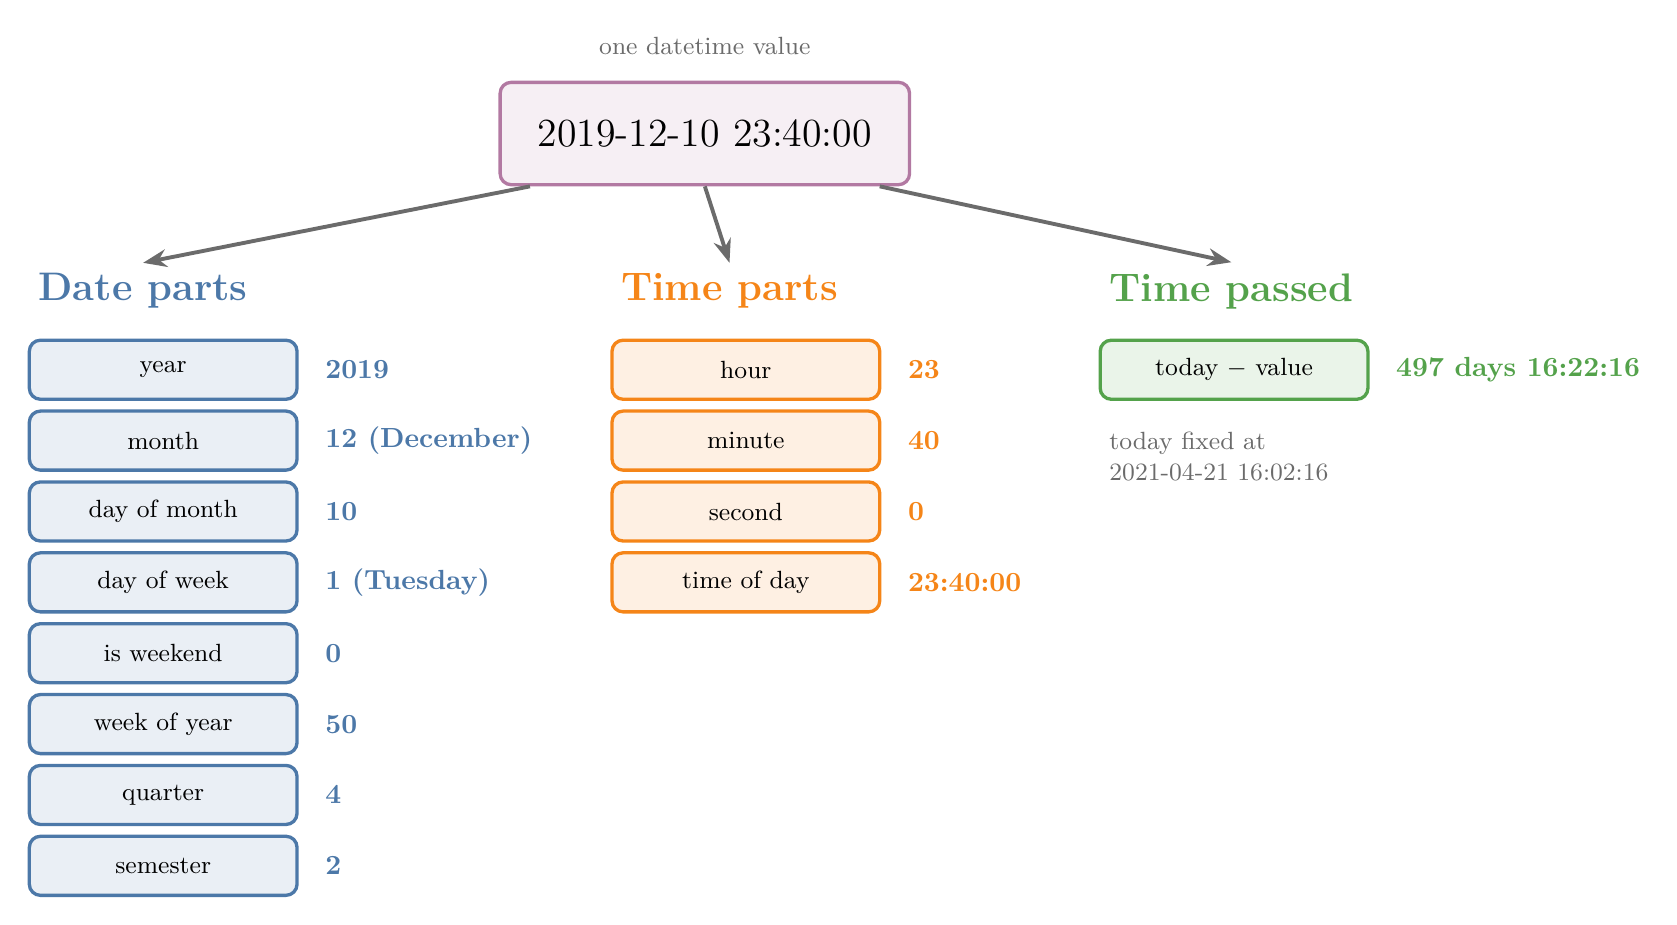
\begin{tikzpicture}
  % the raw value
  \node[box=cpurple, font=\sffamily\Large, minimum width=5.2cm, minimum height=1.3cm] (raw) at (8.6,7.6) {2019-12-10 23:40:00};
  \node[note, above=0.2cm of raw] {one datetime value};
  % group titles
  \node[title, text=cblue, anchor=west] (td) at (0,5.6) {Date parts};
  \node[title, text=corange, anchor=west] (tt) at (7.4,5.6) {Time parts};
  \node[title, text=cgreen, anchor=west] (tp) at (13.6,5.6) {Time passed};
  \draw[arrow] (raw.south west) ++(0.4,0) -- (td.north);
  \draw[arrow] (raw.south) -- (tt.north);
  \draw[arrow] (raw.south east) ++(-0.4,0) -- (tp.north);
  % date parts
  \foreach \y/\n/\v in {4.6/year/2019, 3.7/month/12 (December), 2.8/day of month/10, 1.9/day of week/1 (Tuesday), 1.0/is weekend/0, 0.1/week of year/50, -0.8/quarter/4, -1.7/semester/2}
    { \feat{\y}{0}{\n}{\v}{cblue} }
  % time parts
  \foreach \y/\n/\v in {4.6/hour/23, 3.7/minute/40, 2.8/second/0, 1.9/time of day/23:40:00}
    { \feat{\y}{7.4}{\n}{\v}{corange} }
  % time passed
  \feat{4.6}{13.6}{today $-$ value}{497 days 16:22:16}{cgreen}
  \node[note, anchor=west, align=left] at (13.6,3.5) {today fixed at\\2021-04-21 16:02:16};
\end{tikzpicture}
\end{document}
